\chapter{はじめに}
\label {chp:tex_basic}

\section{研究の背景と目的}
\label{sec:tex_basic_section}
昨今,コロナの影響により,人と直接会う機会が減り,マスクの着用を強いられるようになった.
その結果,笑顔になる機会が減るため,笑顔の減少に繋がる. \\
 しかし,総合人材サービスのパーソルホールディングス株式会社が行った調査[1]では,
仕事をする上で笑顔になると「楽しい」という気持ちが高まった人は約6割で,
ポジティブな感情状態で仕事に取り組んでいた人ほど,笑顔になっており,
職場において笑顔が高まれば,自発的に取り組む傾向があるという結果が出た.

\begin{figure}[!h]
    \begin{center}
        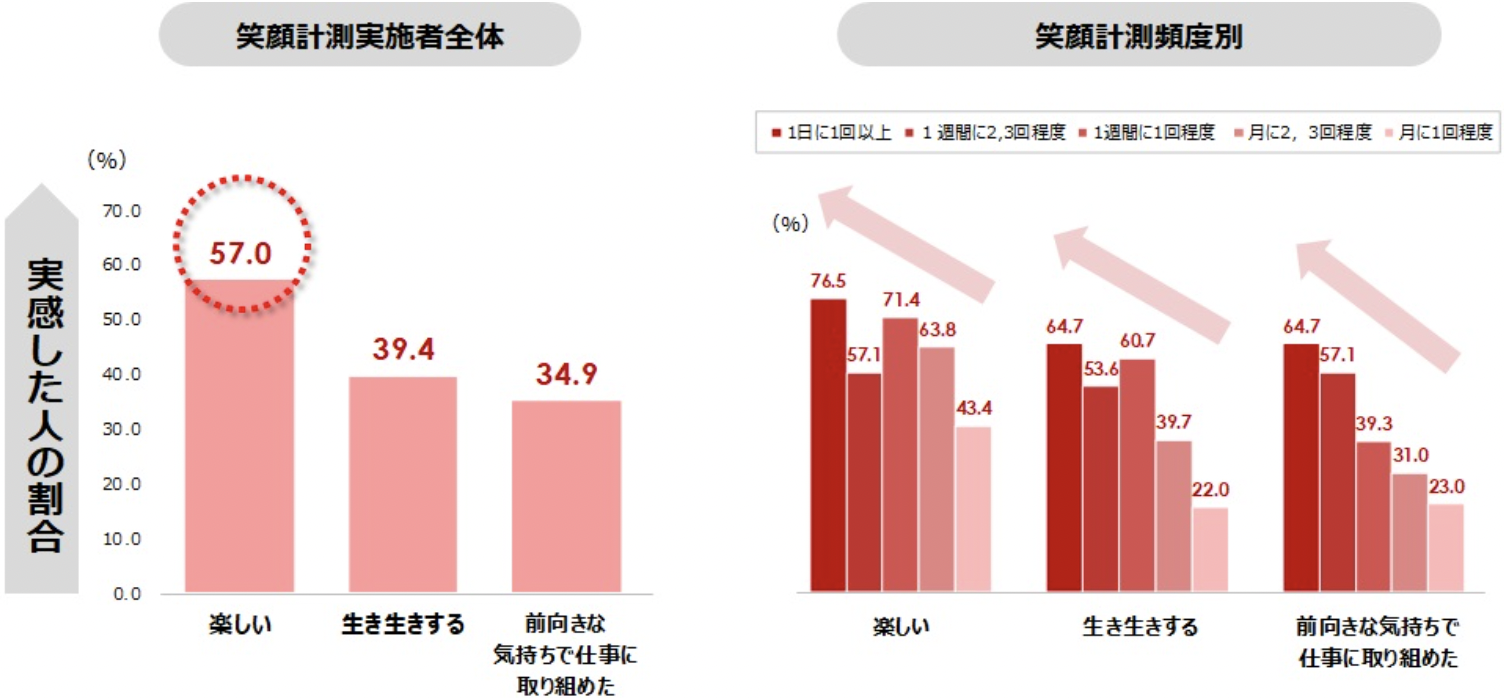
\includegraphics[scale=0.5, clip]{./img/work.png}
        \caption{笑顔計測後の主な感情変化}
        \label{fig:図の名前}
    \end{center}
\end{figure}

また,厚生労働省の調査[2]によると,下のグラフから分かるように,
平成19年度から令和元年にかけて約15\%も増加している.

\clearpage

\begin{figure}[!h]
    \begin{center}
        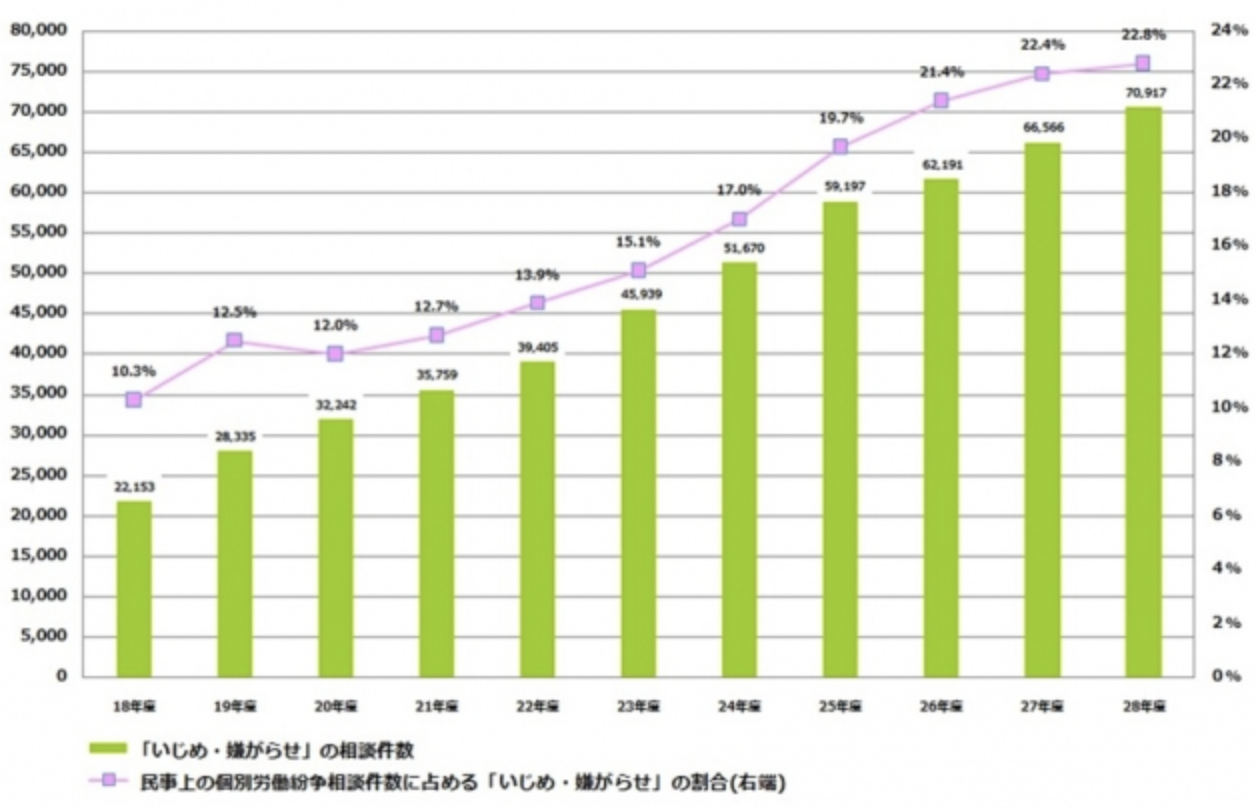
\includegraphics[scale=0.6, clip]{./img/graph.png}
        \caption{厚生労働省によるパワハラ調査}
        \label{fig:図の名前}
    \end{center}
\end{figure}

そこで我々は,以上の課題である「笑顔の減少」と「パワハラの増加」の解決を目的に
FaceAPIを用いた表情分析を活用した労務管理支援システムを提案する.

\section{論文の構成}
\label{sec:tex_basic_newline}
本論文は以下のような構成になっている.
\\
第 1 章では研究背景を述べる.
\\
第 2 章では本研究で開発する労務管理支援システムの概要を述べる.
\\
第 3 章では本研究で開発する労務管理支援システムの構成を述べる.
\\
第 4 章では本研究で開発する労務管理支援システムの実装結果を述べる.
\\
第 5 章では本研究のまとめを述べる.